\documentclass[a4paper,10pt]{article}
\usepackage[margin=2.5cm]{geometry}
\usepackage[utf8]{inputenc}
\usepackage[colorlinks=true,urlcolor=blue]{hyperref}
\usepackage{amsmath}
\usepackage{graphicx}
\usepackage{float}
\usepackage{caption}
\usepackage{xcolor}

\usepackage{listings} %Alternative to minted
\definecolor{codegreen}{rgb}{0,0.6,0}
\definecolor{codegray}{rgb}{0.5,0.5,0.5}
\definecolor{codepurple}{rgb}{0.58,0,0.82}
\definecolor{backcolour}{rgb}{0.95,0.95,0.92}
 
\lstdefinestyle{mystyle}{
    backgroundcolor=\color{backcolour},   
    commentstyle=\color{codegreen},
    keywordstyle=\color{magenta},
    numberstyle=\tiny\color{codegray},
    stringstyle=\color{codepurple},
    basicstyle=\footnotesize,
    breakatwhitespace=false,         
    breaklines=true,                 
    captionpos=b,                    
    keepspaces=true,                 
    numbers=left,                    
    numbersep=5pt,                  
    showspaces=false,                
    showstringspaces=false,
    showtabs=false,                  
    tabsize=2
}

\lstset{style=mystyle}
\setlength{\parindent}{0em}
\setlength{\parskip}{1em}

\title{\textbf{Deep Learning for Image Analysis} 
\\ DL4IA -- Report for Assignment 1}
\author{Student Linus Falk}
\date{\today}

\begin{document}
\lstset{language=Python}
\maketitle

\section{Introduction}
First assignment in the course Deep learning for image analysis

\section{Mathematical exercises}

Given the linear regression model:
\begin{equation}
    z_i = \sum_{j=1}^p w_jx_{ij} + b 
\end{equation}

with the cost function 
\begin{equation}
\label{eq:cost}
\begin{split}
    J = \frac{1}{n}\sum_{i=1}^nL_i \\
    \text{where } L_i = (y_i-z_i)^2    
\end{split}
\end{equation}



\textit{\textbf{Exercise 1.}}
\begin{equation*}
    \frac{\partial J} {\partial w_j} = \frac{1} {n} \sum_{i=1}^{n} \frac{\partial J} {\partial z_i}  \frac{\partial z_i} {\partial w_j} 
\end{equation*}

\begin{equation*}
   \frac{\partial J} {\partial b}  = \frac{1} {n} \sum_{i=1}^{n} \frac{\partial J} {\partial z_i}  \frac{\partial z_i} {\partial b} 
\end{equation*}


\textit{\textbf{Exercise 2.}}

\begin{equation*}
\begin{split}
    \frac{\partial J}{\partial z_i} = \frac{1} {n} \sum_{i=1}^{n}  2(y_i-z_i) \\
    \frac{\partial z_i} {\partial b} = \frac{\partial} {\partial b}  \sum_{j=1}^p (w_jx_{ij}+b) = 1 \\
    \frac{\partial z_i} {\partial w_j} = \frac{\partial} {\partial w_j} \sum_{j=1}^p (w_jx_{ij}+b) = \sum_{j=1}^p x_{ij}
\end{split}
\end{equation*}


\section{Code exercises}

\hfill \break
\textit{\textbf{Exercise 3.} Implement a gradient descent algorithm ...}

Based on the derivations given in exercise 1 and 2, the following functions are implemented to perform gradient descent for linear regression. 

\begin{itemize}
\item
The \emph{initiliaze\_parameters} function is used to initialize the weights and offsets by method X.
\item
The \emph{compute\_cost} function takes Y\_pred and Y as input and calculates the cost according to eq. \eqref{eq:cost}.
\item The \emph{model\_forward} function takes the input features and compute the predictions with the weight and bias/offset
\end{itemize}

\begin{lstlisting}

class NeuralNetwork:
    # Create a neural network with #hidden layers and #neurons in each layer
    def __init__(self, features, learningRate, *args):
    """ param features: number of features in the input
        param learningRate: set the learningrate/stepsize
        param *args: number of hidden nodes
        
        return: Creates a linear regression node for now 
    """
        self.features = features
        self.args = args
        self.learningRate = learningRate
        self.weights = None
        self.bias = None
        self.dW = None
        self.dB = None
        self.training_history = []


    def initiliaze_parameters(self):
    """ 
        return: returns a weight array with zeros \\
        according to the input size and a bias variable set to zero
    """

    self.weights = np.zeros((self.features,1))
    self.bias = 0
    
    
    return w, b

    def compute_cost(self, Y_pred, Y):
    """ param Y_pred: prediction of Y after forward pass
        param Y: the label
        ...
        
        return: the cost
    """ 
        return (Y_pred - Y)

    def model_forward(self, X):
    """...       
        return: the prediction with this set of weight and bias
    """ 
        y_pred = np.dot(X, self.weights) + self.bias
        return y_pred

    #Forward run wrapper
    def predict(self, X):
        return self.model_forward(X)


\end{lstlisting}

\newpage
\hfill \break
The weights and offsets are optimized to minimize the cost as follows:
\begin{itemize}
\item
The \emph{train\_linear\_model} function is used to train a linear model with given input X and labels Y with the given number of iterations. 
\item
The \emph{model\_backward} function computes the forward pass first to have a new prediction of Y to calculate the cost. It then computes the gradients.
\item The \emph{update\_parameters} function takes a step with the calculated gradients and updates the weight and biases. 
\end{itemize}


\begin{lstlisting}
    #Train the network
    def train_linear_model(self, X, Y, iterations):
    """ param X: the input X we want to forward
        param Y: the label
        param iteration: number of training iteration
        ...
    """
        for i in range(iterations):
            nn.model_backward(X, Y)
            nn.update_parameters()


    #Calculate the gradients 
    def model_backward(self, X, Y):
    """ param X: the input X we want to forward
        param Y: the label
        ...
        return: 
    """ 
        samples, features = X.shape
        Y_pred = self.model_forward(X)
        cost = self.compute_cost(Y_pred, Y)
        
        self.dW = (2/samples) * np.dot(X.T, cost) 
        self.dB = (2/samples) * np.sum(cost)
        self.training_history.append(np.mean(np.abs(cost)))


    #Update the weight and bias with the pre-calculated gradients
    def update_parameters(self):
        self.weights -= self.learningRate * self.dW
        self.bias -= self.learningRate * self.dB



\end{lstlisting}


\section{Results}

Here follows the mathematical expression \eqref{eq:model} of the two trained models. Taking a look at the model with seven inputs we can see that it put more weight into the features: \textbf{weight} and \textbf{year}. This makes a lot of sense. Since the weight will greatly affect the fuel consumption in a mixed driving situation, accelerating more mass require more fuel. The year is also highly relevant since the car manufacturers has become better and better producing efficient engines. 


\begin{equation}
\begin{aligned}
    \textbf{W}_{\text{all features}}^{T}\textbf{x} + \textbf{b}_{\text{all features}} = \begin{bmatrix} -1.20 \\ -0.18 \\ -1.96 \\ -16.84 \\ 0.92 \\ 8.87 \\2.65 \end{bmatrix}^{T}\begin{bmatrix} \text{cylinders}\\\text{displacement}\\ \text{horsepower}\\ \text{weight} \\  \text{acceleration} \\ \text{year} \\ \text{origin} \end{bmatrix} + \begin{bmatrix} 25.63 \end{bmatrix} = \begin{bmatrix} \text{mpg} \end{bmatrix} \\
   \\
    \textbf{W}_{\text{one feature}}^{T}\textbf{x} +\textbf{b}_{\text{one feature}} = \begin{bmatrix} -29.03 \end{bmatrix} \begin{bmatrix} \text{horsepower} \end{bmatrix} +\begin{bmatrix} 32.67 \end{bmatrix}  = \begin{bmatrix} \text{mpg} \end{bmatrix}
\label{eq:model}
\end{aligned}
\end{equation}

The training history is presented in figure \ref{fig:cost_per_iteration}. Learning rate 1 was neglected since it is to big of a step and diverges. We can see that the small steps takes longer time to converge and that the model with one feature don't manage to achieve the same low cost as the model with more features. This is because there are more information in the model with seven features available and can therefore make better predictions. More is not always better though, fitting a model to a feature data with poor resolution that is included can result in worse performance than if that feature was discarded. Taking a look at the predictions of the model with one feature: \textbf{horsepower} vs the label \textbf{mpg} and plotting the training data we can see that it has fitted the line as expected to the data, see figure \ref{fig:hpvsmpg}. 

In the case of not normalizing the input we must decrease the step size considerably before it can converge and it will take considerably more steps until we get decent performance in comparison with using normalized data, see figure \ref{fig:nonorm}. 

\begin{figure}[H]
 \centering
    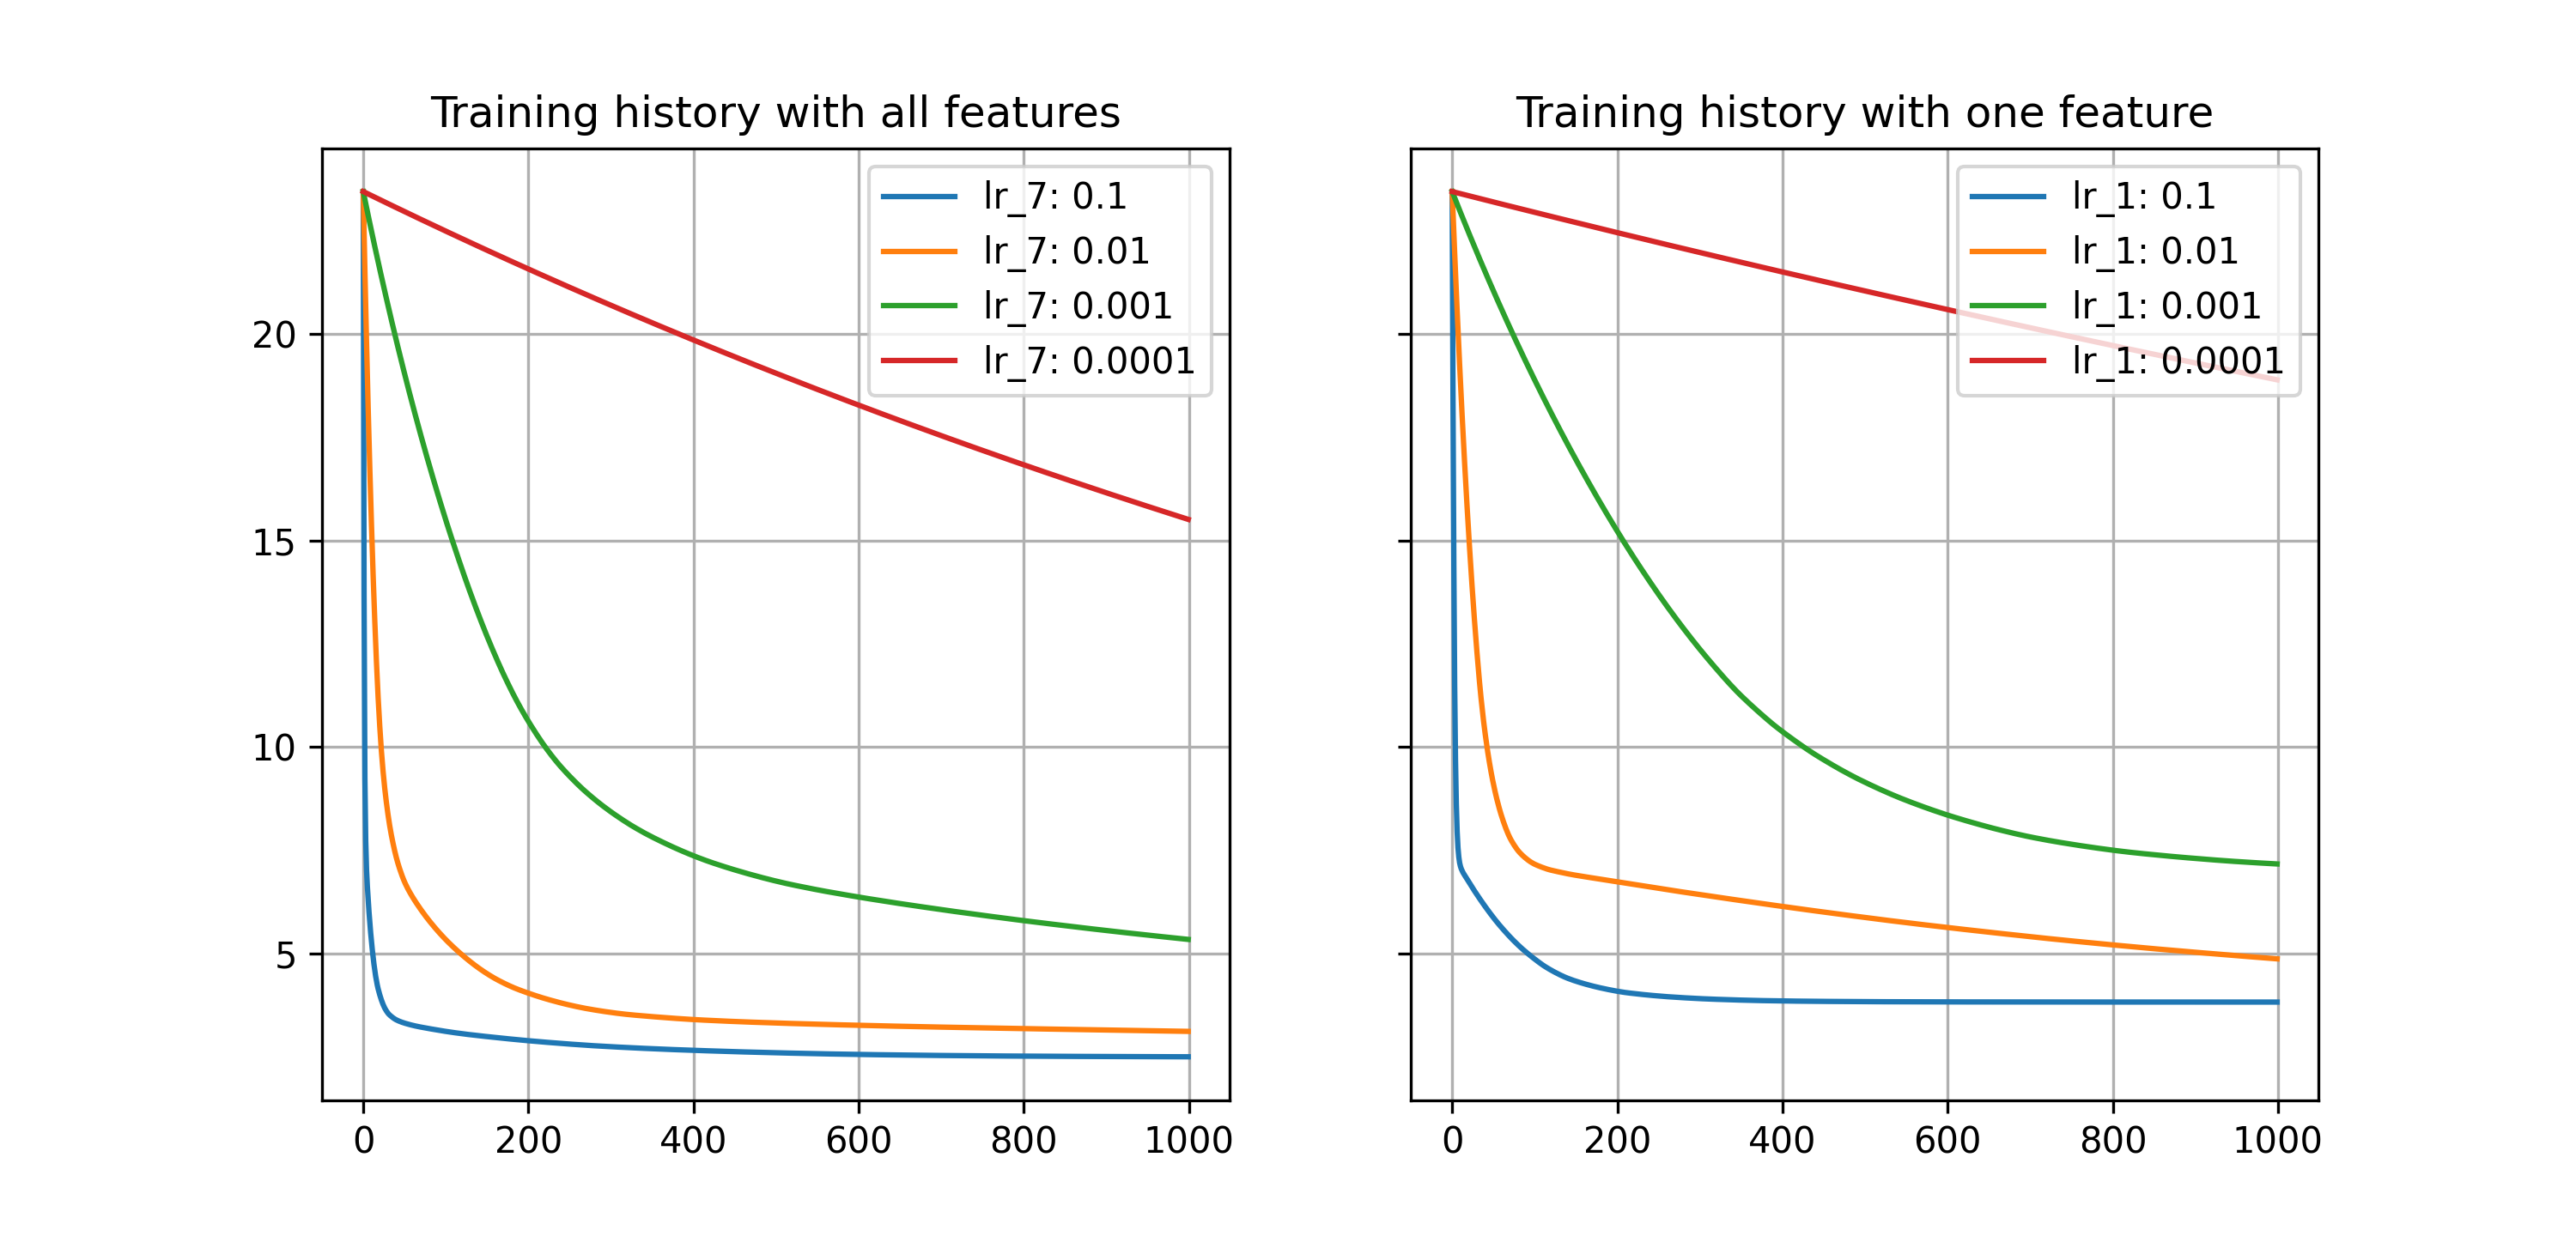
\includegraphics[width=0.8\textwidth]{figures/all_one_feature.png}
    \caption{Plot showing how the cost \eqref{eq:cost}, evaluated on the training sets, is changing with with number of iterations}
    \label{fig:cost_per_iteration}
\end{figure}

\begin{figure}[H]
 \centering
    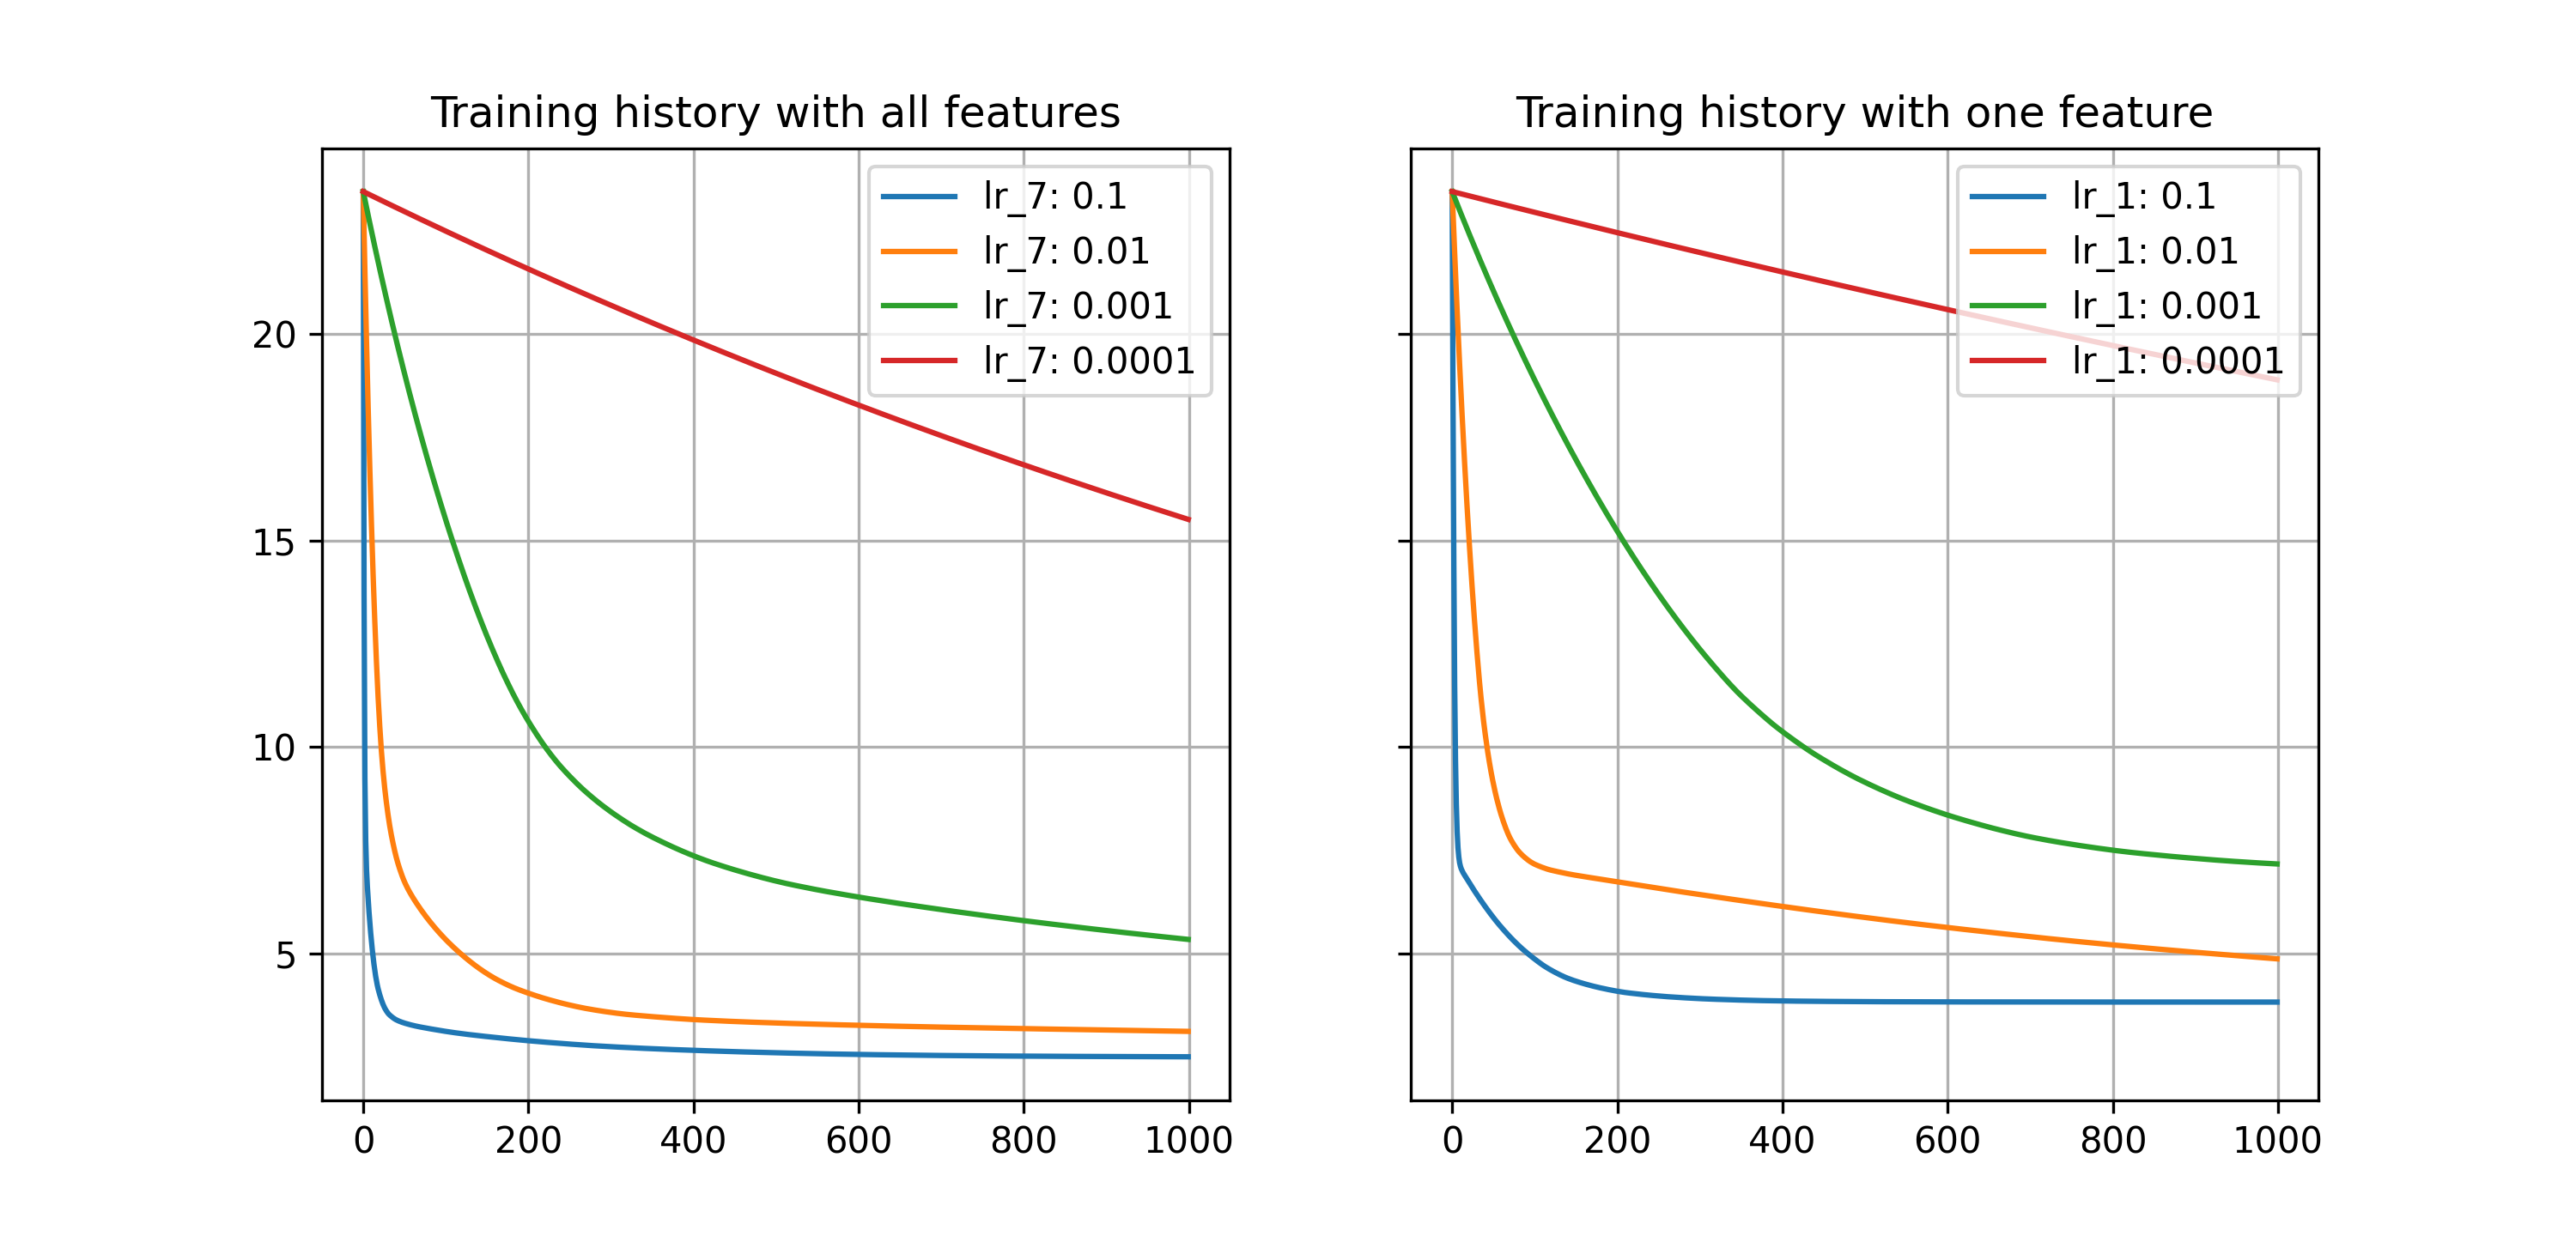
\includegraphics[width=0.8\textwidth]{figures/no_norm.png}
    \caption{Plot showing how the cost \eqref{eq:cost}, evaluated on the \textbf{non normalized} training sets, is changing with with number of iterations}
    \label{fig:nonorm}
\end{figure}

\begin{figure}[H]
 \centering
    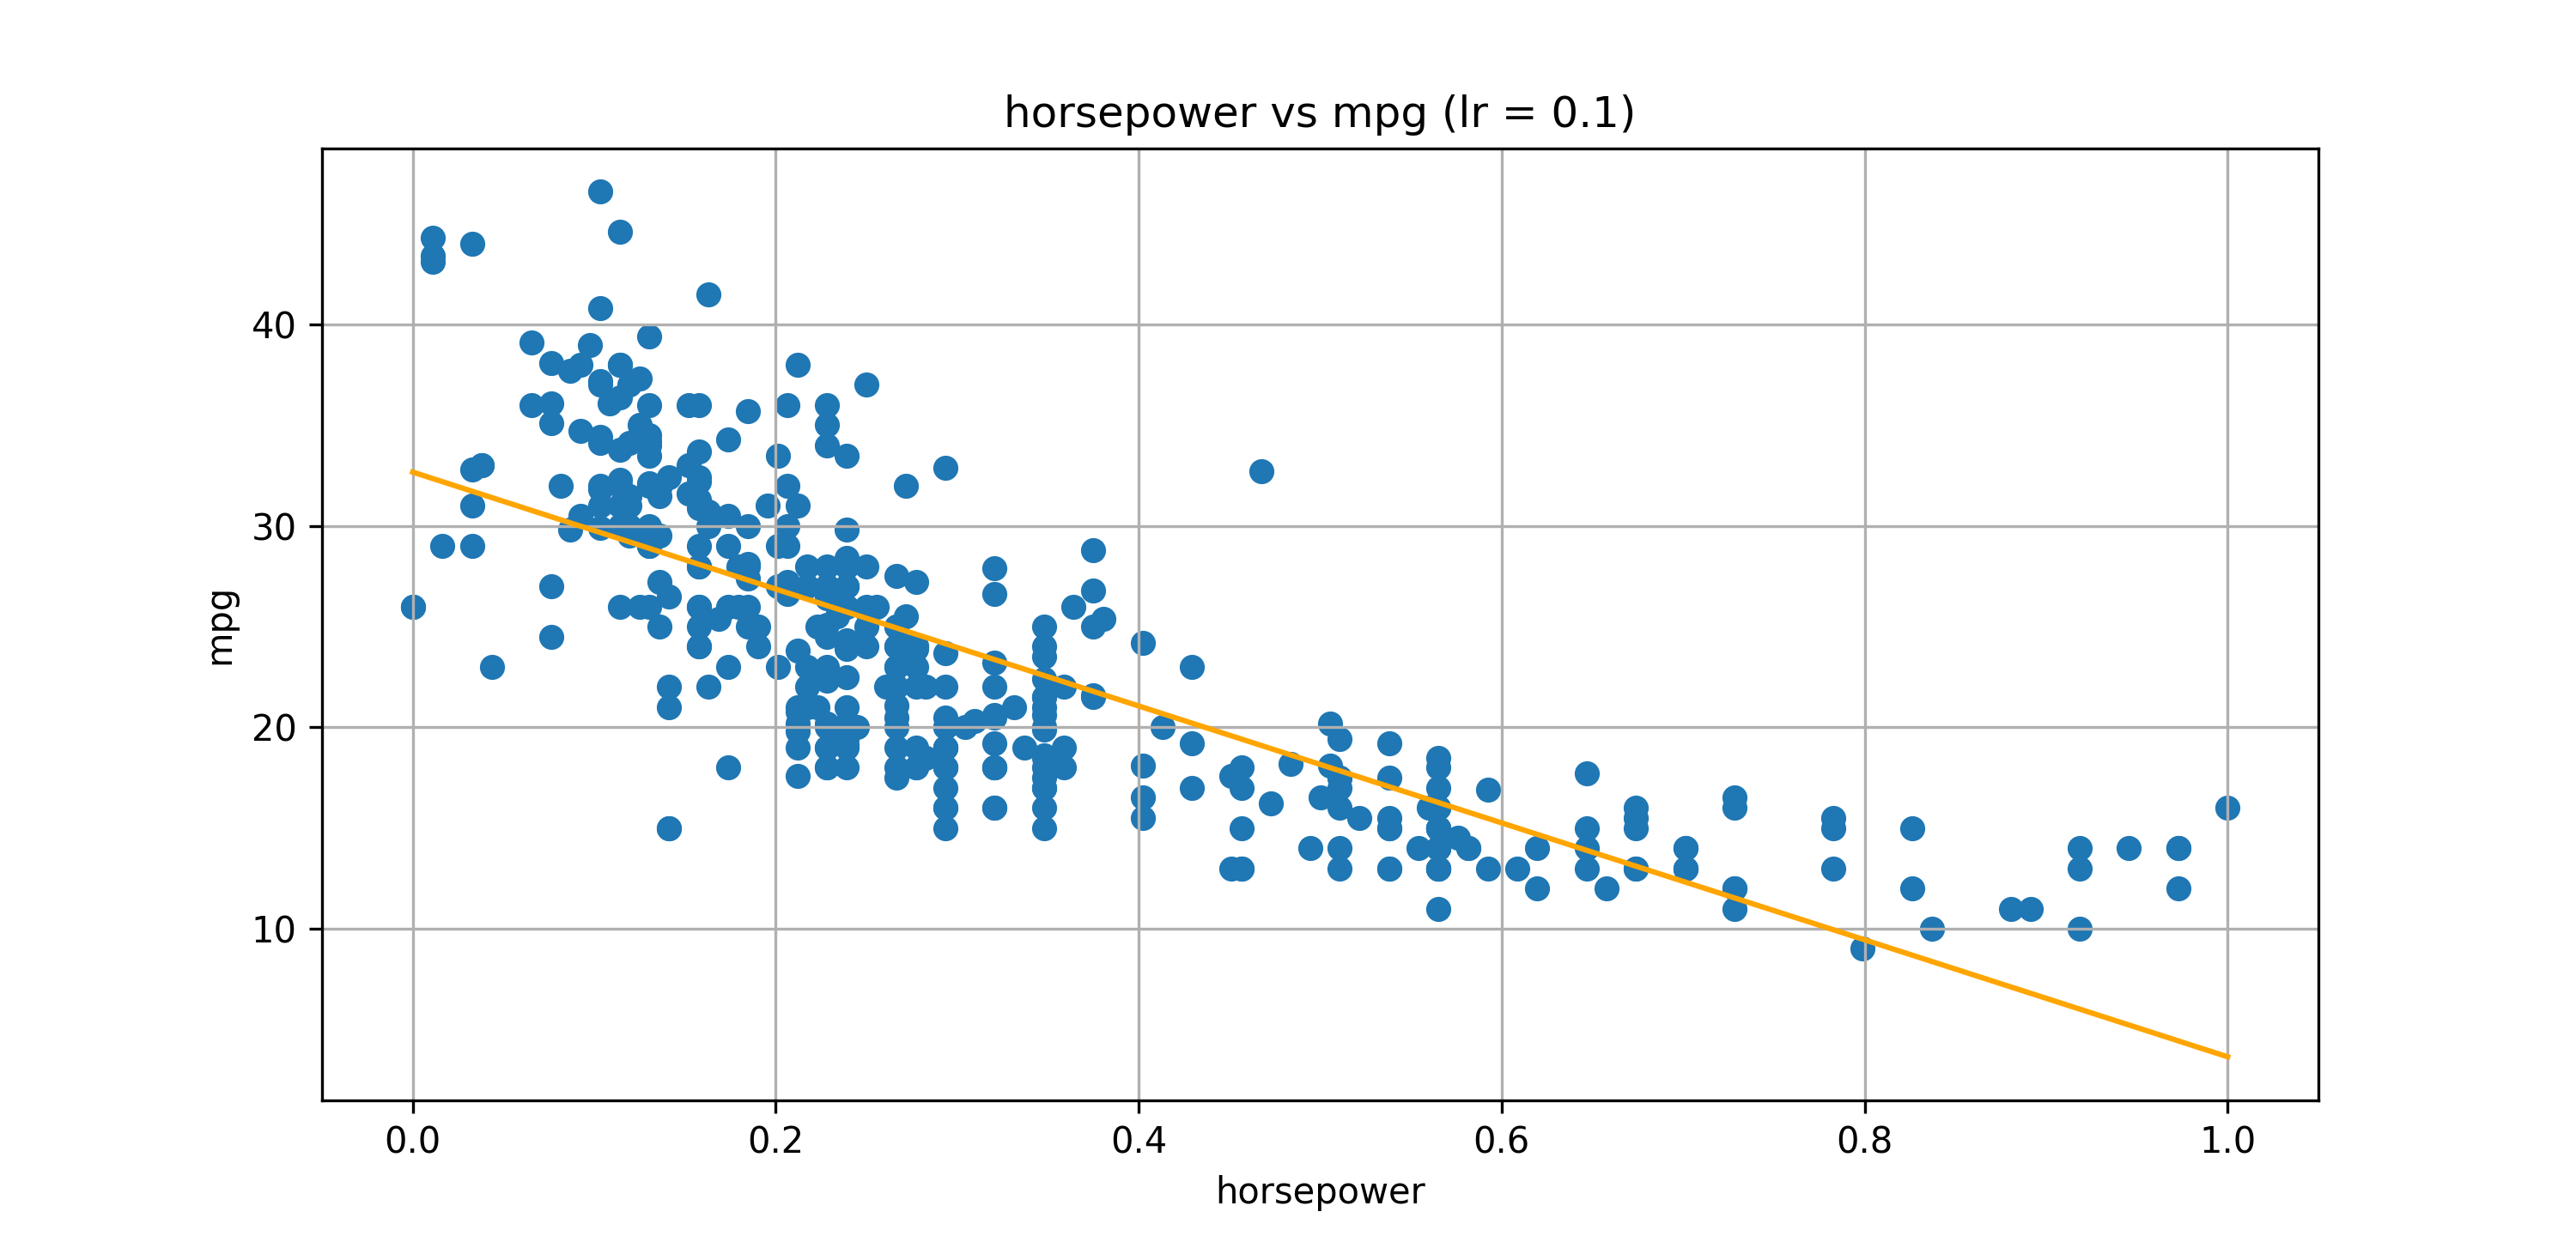
\includegraphics[width=0.8\textwidth]{figures/hp_mpg.png}
    \caption{Plot showing the model with horsepower as the only input}
    \label{fig:hpvsmpg}
\end{figure}


\begin{thebibliography}{1}

\bibitem{Asimov} Asimov, Issac (1942). Runaround

\end{thebibliography}

\end{document}
